% ACL Rolling Review long paper: 8 pages of content; Limitations, Ethical Considerations, references and appendices
% do not count. Template: official *ACL style files, unmodified.
% Figures and tables: ../scripts/figs_v3.py (computed from the result files in ../results).
\documentclass[11pt]{article}

\usepackage[review]{acl}
\usepackage{times}
\usepackage{latexsym}
\usepackage[T1]{fontenc}
\usepackage[utf8]{inputenc}
\usepackage{microtype}
\usepackage{inconsolata}
\usepackage{graphicx}
\usepackage{booktabs}
\usepackage{makecell}
\usepackage{amsmath,amssymb}
\usepackage{xcolor}
\usepackage[inline]{enumitem}

\newcommand{\head}[1]{\texttt{#1}}

\title{Which Head Does the Work? How Attention-Head Circuit Findings\\ Carry Over Between Related Language Models}

\author{Anonymous ACL submission}

\begin{document}
\maketitle

\begin{abstract}
Circuit analyses name the attention heads that carry a computation, and these names are routinely reused: on later checkpoints, on fine-tuned descendants, and on sibling models trained from the same initialization on other data.
We ask in which related models the named heads actually do the work.
Using public model suites that cross initialization with training data (69 DataDecide models at 1B parameters on 25 corpora; Pythia 160M--12B and its deduplicated sibling), the full OLMo~2 lineage from pretraining through midtraining, SFT, DPO and instruction tuning, and controlled pretraining, we separate three things that a head-level finding can mean.
The layer that hosts a role and the algorithm a circuit runs are shared by all models.
The attention role of an individual head is shared among models trained from the same initialization, across all 25 corpora, and not between models from different initializations.
The causal carrier of a task is assigned by training: siblings that share the initialization and differ only slightly in data run the same indirect-object-identification algorithm on different heads, while a model's own carriers, once settled in pretraining, stay in place through midtraining, preference tuning and instruction tuning.
Controlled pretraining exposes the mechanism: the heads of a functional class compete for a role while it forms, and when two candidates are close, masking a random 10\% of the data hands the role to the other one with the ability intact.
Head-level findings therefore carry over along a training lineage, and attention-role labels carry over within an initialization; across separately trained runs, the algorithm carries over and the carriers are found anew.
\end{abstract}

\section{Introduction}

Mechanistic interpretability explains a computation by locating the components that carry it.
A circuit for indirect-object identification (IOI) is a set of named heads, \emph{e.g.}, the name movers and the heads that suppress the repeated name \citep{wang2023interpretability}; an induction circuit is a previous-token head composed with an induction head \citep{olsson2022context}.
Such findings are then used beyond the model in which they were found.
Circuits are tracked across the checkpoints of a training run \citep{tigges2024llm}, compared between a base model and its fine-tuned versions \citep{prakash2024finetuning}, and used as the target of training-data interventions that retrain a model and read out the same head again \citep{chen2026mechanistic}.
Each of these uses assumes that a specific head in one model corresponds to a specific head in another.

Which correspondences hold is not determined by the architecture.
Heads within a layer are interchangeable: permuting them, together with their output projections, leaves the function unchanged, so a head's index carries meaning only relative to a particular training history.
Prior work has shown that circuits are consistent in their algorithm across training and scale while their components change \citep{tigges2024llm}, that individual heads are unstable across random seeds \citep{bali2026quantifying}, and that positional agreement across Pythia seeds is limited \citep{trott2025generalizability}.
These studies vary the seed, which changes the initialization and the data order together, and they compare runs that were trained separately.
The uses listed above, however, involve two other relations between models: siblings that share an initialization but see different data, and descendants that continue the training of the same model.

We separate the relations with populations in which they can be varied one at a time (\S\ref{sec:setup}).
DataDecide crosses three initializations with 25 pretraining corpora at 1B parameters \citep{magnusson2025datadecide}; Pythia releases a standard and a deduplicated model from the same initialization at every size, with intermediate checkpoints \citep{biderman2023pythia}; OLMo~2 releases every stage of one lineage from pretraining to instruction tuning \citep{olmo2024olmo2}; and controlled pretraining lets us intervene on the data of a single run.
In each model we measure attention roles of every head and the causal carriers of IOI, with split-half reliability for every head map.

Three findings organise the paper.
\begin{enumerate*}[label=(\arabic*)]
\item \textbf{Initialization fixes a shared coordinate system} (\S\ref{sec:roles}).
All models agree on the layer that hosts each of nine head roles; which head within the layer takes the role is shared by all models from the same initialization across 25 corpora and by no other model.
\item \textbf{Training assigns the causal carriers within that coordinate system} (\S\ref{sec:carriers}).
Siblings from the same initialization run the same IOI algorithm with different heads, including siblings whose corpora differ only by the removal of 1.5\% of the data, and, at four of six Pythia sizes, by deduplication.
\item \textbf{Carriers move during pretraining and then stay} (\S\ref{sec:lineage}).
Along one run, responsibility moves among heads of the same functional class through most of pretraining, and the carriers present at the end of pretraining are the carriers after midtraining, SFT, DPO and instruction tuning.
\end{enumerate*}
Controlled pretraining shows the competition directly (\S\ref{sec:masking}): when one induction head leads, masking training data during its emergence delays that head; when two heads are nearly equal, masking a random 10\% of the data hands the role to the other head with the ability intact.

These findings give a practical rule (\S\ref{sec:discussion}): a head-level finding carries over along a training lineage; an attention-role label carries over within an initialization; across separately trained runs the algorithm carries over and the carriers are localized again.
Along the way, the head layouts identify four public checkpoints whose lineage differs from their labels, including the released OLMo-2-1B base model (Appendix~\ref{app:audit}).

\section{Setup}
\label{sec:setup}

\paragraph{Model populations.}
\emph{DataDecide-1B} trains three initializations (seeds \texttt{default}, \texttt{large-aux-2}, \texttt{large-aux-3}) on 25 corpora for 100B tokens \citep{magnusson2025datadecide}.
We verified every run's initialization against the released step-0 weights and use the 69 runs whose initialization matches its label (Appendix~\ref{app:audit}).
Pairs of runs are either \emph{siblings} (same initialization, different corpus) or \emph{unrelated} (different initialization).
\emph{Pythia} trains a standard and a deduplicated model from the same initialization at each size \citep{biderman2023pythia}; we use 160M to 12B and fifteen checkpoints of the 160M and 410M pairs.
\emph{OLMo-2-0425-1B} provides one lineage: the end of pretraining (4T tokens), three midtraining runs on different mixtures (51B tokens each), and the SFT, DPO and Instruct models \citep{olmo2024olmo2}.
\emph{Controlled pretraining} trains 12-layer, 12-head Llama-style models on C4 from three initializations with a fixed data order (Appendix~\ref{app:controlled}).

\paragraph{Attention roles.}
For every head we compute nine role scores \citep{olsson2022context,xiao2024efficient,wu2025retrieval}: induction, previous token, attention sink, knowledge retrieval, duplicate token, current token, two tokens back, delimiter, and a weight-only OV copying score (Appendix~\ref{app:roles}).
Each score gives a [layer $\times$ head] map per model.

\paragraph{Causal carriers of IOI.}
We use the IOI dataset of \citet{wang2023interpretability} (200 prompts, mixed templates) and, for every head, (i) its direct logit attribution to the IO name over the subject name at the final position, with every normalization linearized at its actual scale, (ii) the drop in logit difference when the head's input to the output projection is mean-ablated at the final position, and (iii) its attention from the final position to the IO and S2 tokens.
The carriers of a model are its heads with the largest direct effect; we compare carriers between models by the overlap of their top three heads and by \emph{transfer}, the damage that ablating one model's top-three heads does in the other model relative to the other model's own top three.

\paragraph{Comparing head maps.}
Two models' maps are compared within each layer by rank correlation, averaged over layers, so that agreement on which layer hosts a role does not count as agreement on which head does.
Every map is computed on two halves of its inputs, and correspondences between models are divided by the geometric mean of the two models' split-half reliabilities.
This matters for causal maps: most heads contribute nothing to IOI, so a rank correlation over all heads in a layer is dominated by the order of near-zero values and reaches a split-half reliability of only 0.40--0.50 for direct logit attribution, although the values of the contributing heads replicate almost perfectly (0.98).
Single-head ablation maps are reliable under the rank statistic (0.83--0.86) and are our causal map; carrier identity and transfer use the contributing heads directly (Table~\ref{tab:reliability}).

\begin{table}[t]
\centering\small
\setlength{\tabcolsep}{3pt}
\resizebox{\columnwidth}{!}{\begin{tabular}{lccccc}
\toprule
& induction & END$\to$IO & ablation & DLA (rank) & DLA (value) \\
\midrule
DataDecide-1B (9 models) & 1.00 & 0.99 & 0.83 & 0.50 & 0.98 \\
Pythia-410M & 0.99 & 0.99 & 0.83 & 0.40 & 0.99 \\
OLMo-2-1B (pretraining end) & 1.00 & 0.99 & 0.86 & 0.42 & 0.98 \\
\bottomrule
\end{tabular}
}
\caption{Split-half reliability of head maps (Spearman--Brown corrected).
Rank statistics are reliable for attention maps and ablation maps; for direct logit attribution (DLA) the values of the contributing heads are reliable, while the ranks of the many near-zero heads are not.}
\label{tab:reliability}
\end{table}

\section{Initialization fixes a coordinate system}
\label{sec:roles}

\begin{table}[t]
\centering\small
\setlength{\tabcolsep}{3.2pt}
\resizebox{\columnwidth}{!}{\begin{tabular}{lcccc}
\toprule
& \multicolumn{3}{c}{which head within the layer} & which layer \\
\cmidrule(lr){2-4}\cmidrule(lr){5-5}
Role & \makecell{same init.\\diff.\ corpus} & \makecell{diff.\ init.\\same corpus} & \makecell{both\\differ} & \makecell{same init.\ /\\both differ} \\
\midrule
Induction & 0.33 & -0.02 & 0.00 & 0.49 / 0.41 \\
Previous token & 0.42 & -0.01 & -0.00 & 0.46 / 0.38 \\
Attention sink & 0.18 & -0.01 & -0.00 & 0.64 / 0.58 \\
Knowledge retrieval & 0.31 & -0.00 & 0.00 & 0.60 / 0.54 \\
Duplicate token & 0.36 & -0.02 & -0.01 & 0.62 / 0.57 \\
Current token & 0.32 & -0.02 & -0.00 & 0.61 / 0.59 \\
Two tokens back & 0.43 & -0.00 & 0.01 & 0.62 / 0.58 \\
Delimiter & 0.22 & -0.01 & 0.00 & 0.57 / 0.50 \\
OV copying (weights only) & 0.25 & -0.01 & -0.01 & 0.68 / 0.64 \\
\bottomrule
\end{tabular}
}
\caption{Correspondence of head-role maps across the 69 DataDecide-1B models.
Which head within a layer takes a role is shared by siblings (same initialization, different corpus) and by no other pair; the profile over layers is shared by every pair.}
\label{tab:roles}
\end{table}

\begin{figure}[t]
\centering
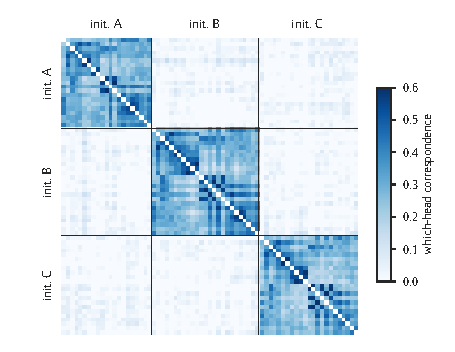
\includegraphics[width=\columnwidth]{figures/fig_maps}
\caption{Which-head correspondence between all pairs of the 69 DataDecide-1B models (mean within-layer correspondence of four attention roles), ordered by initialization and, within each block, by corpus.
Models from one initialization form one block across all 25 corpora.}
\label{fig:maps}
\end{figure}

Across the 69 DataDecide-1B models, the layer profile of every role is shared by all pairs of models, related or not, and which head inside the layer takes the role follows the initialization (Figure~\ref{fig:maps}, Table~\ref{tab:roles}).
Ordered by initialization, the pairwise correspondences form three blocks: siblings correspond at 0.31 on average and models from different initializations at 0.00, and the two distributions barely touch (lowest sibling pair 0.10, highest unrelated pair 0.14).
Siblings trained on different corpora agree on the head for every one of the nine roles (within-layer correspondence 0.18--0.43), whereas models from different initializations agree at chance whether they share the corpus or not.
A per-head variance decomposition makes the same point: the initialization has a significant effect on 66--79\% of heads for the attention roles, the corpus on 4--7\%, the rate expected by chance.
The weight-only OV copying score behaves like the attention roles, so the shared assignment is a property of the weights and not of the probe inputs.

\begin{figure}[t]
\centering
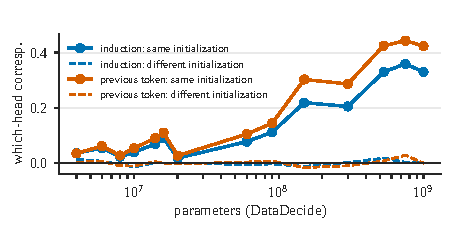
\includegraphics[width=\columnwidth]{figures/fig_scale}
\caption{The shared coordinate system across 14 DataDecide sizes: within-layer correspondence of induction and previous-token maps between siblings (solid) and between models from different initializations (dashed).}
\label{fig:scale}
\end{figure}

The coordinate system strengthens with scale (Figure~\ref{fig:scale}).
Across the 14 DataDecide sizes, sibling correspondence is small below 20M parameters, clear from 60M, and reaches 0.33--0.44 at 0.5--1B, while models from different initializations stay at zero at every size.

The initialization therefore defines a coordinate system that all its descendants share: in two siblings, ``layer 12, head 3'' refers to a head with the same attention role, and component-level comparisons between siblings need no alignment.
This holds across all 25 corpora, which range from web crawls to curated and quality-filtered mixtures.

\section{Training assigns the carriers}
\label{sec:carriers}

\begin{figure}[t]
\centering
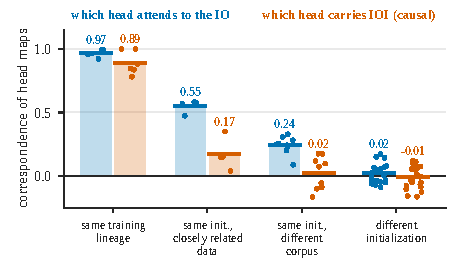
\includegraphics[width=\columnwidth]{figures/fig1_carryover}
\caption{What carries over between two models, by their relation.
Blue: correspondence of the attention map from the final position to the IO name; orange: reliability-corrected correspondence of the single-head ablation map for IOI.
Bars are means over model pairs, whiskers the range.
Siblings share the attention role of a head but not its causal role; models in one training lineage share both.}
\label{fig:carryover}
\end{figure}

Within the shared coordinate system, a task's causal carriers are a separate matter (Figure~\ref{fig:carryover}).
For IOI, the attention role of a head, whether it attends from the final position to the IO name, corresponds between DataDecide siblings at 0.24, the same level as the roles of \S\ref{sec:roles}.
The causal map does not: its reliability-corrected correspondence between siblings is 0.02, as low as between models with different initializations (0.01), and the top-three carriers of one sibling transfer 3\% of the damage to another.
Of the 18 sibling pairs among four DataDecide corpora, none share the main carrier.

The assignment is equally independent of how similar the data are.
Removing the Flan instruction data, about 1.5\% of the Dolma corpus, gives three sibling pairs whose attention roles agree most closely of all the sibling pairs we compare (0.57--0.58), and each pair carries IOI on different main heads.
The standard and deduplicated Pythia models carry IOI on largely the same heads at 160M and 1B (transfer 0.85 and 0.90) and on different heads at 410M, 1.4B, 6.9B and 12B (transfer between $-$0.05 and 0.16; Table~\ref{tab:pythia}); at 410M their attention roles still correspond at 0.48 while their causal maps correspond at 0.15.

\begin{table}[t]
\centering\small
\resizebox{\columnwidth}{!}{\begin{tabular}{lcccc}
\toprule
Size & \makecell{main carrier\\(standard)} & \makecell{also in sibling's\\top three} & \makecell{top-3\\shared} & transfer \\
\midrule
160M & 8.9 & yes & 2/3 & 0.85 \\
410M & 11.4 & no & 0/3 & 0.05 \\
1B & 12.1 & no & 0/3 & 0.90 \\
1.4B & 10.7 & no & 0/3 & -0.05 \\
6.9B & 20.28 & no & 0/3 & 0.04 \\
12B & 20.11 & no & 0/3 & 0.16 \\
\bottomrule
\end{tabular}
}
\caption{IOI carriers of standard and deduplicated Pythia models (same initialization).
Transfer: damage of the standard model's top three heads in the deduplicated model, relative to the latter's own top three.}
\label{tab:pythia}
\end{table}

What differs is the head, not the computation.
In the Pythia models we analysed head by head (160M and 410M, standard and deduplicated, and an independently initialized 410M), IOI runs on the same functional classes: a head that attends to the repeated subject and writes against it through a negative OV copying circuit, and several name movers that attend to the IO name and copy it \citep{wang2023interpretability}.
Each class has several members in each model, and siblings give the main role to different members (Figure~\ref{fig:classes}).
In the 410M Pythia pair, the strongest carrier of the standard model, \head{11.4}, contributes 1.16 to the logit difference and its counterpart in the deduplicated model 0.02, while the deduplicated model's strongest carrier, \head{12.12}, contributes 0.97 and its counterpart 0.00; each is nearly silent in the other model, attending to the first token instead.

\begin{figure}[t]
\centering
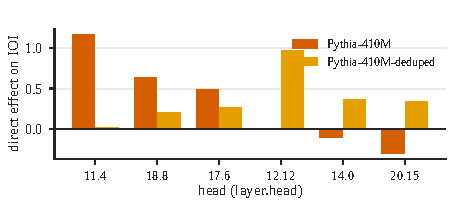
\includegraphics[width=\columnwidth]{figures/fig_classes}
\caption{Same algorithm, different carriers.
Direct effect on the IOI logit difference of each sibling's top-three heads, measured in both siblings (Pythia-410M and its deduplicated version, same initialization).
Each model's main carrier is silent in the other.}
\label{fig:classes}
\end{figure}
Because several heads in a class share the attention profile, attention and OV profiles do not determine which member carries the task: mapping one model's carriers onto the other by these profiles recovers between 106\% and $-$6\% of the target's own top-three damage depending on the pair, whereas a causal readout in the target recovers 85--94\%.
The carrier has to be identified causally in each model.

\section{Carriers move during pretraining, then stay}
\label{sec:lineage}

\begin{table}[t]
\centering\small
\setlength{\tabcolsep}{2.6pt}
\resizebox{\columnwidth}{!}{\begin{tabular}{lccccc}
\toprule
& \makecell{attention\\role} & \makecell{ablation\\map} & \makecell{top-3\\carriers} & transfer & \makecell{main\\carrier} \\
\midrule
Pretraining end $\to$ midtraining, 5B tokens & 0.96 & 0.85 & 2/3 & 0.93 & 14.4 \\
Pretraining end $\to$ midtraining mix 1, 51B & 0.96 & 0.84 & 2/3 & 0.94 & 14.4 \\
Pretraining end $\to$ midtraining mix 2, 51B & 0.96 & 0.85 & 2/3 & 0.95 & 14.4 \\
Pretraining end $\to$ midtraining mix 3, 51B & 0.96 & 0.88 & 2/3 & 0.94 & 14.4 \\
SFT $\to$ DPO & 0.99 & 1.00 & 3/3 & 1.00 & 14.4 \\
DPO $\to$ Instruct & 1.00 & 1.00 & 3/3 & 1.00 & 14.4 \\
Pythia-410M step 66k $\to$ 143k & 0.92 & 0.78 & 3/3 & 0.99 & 11.4 \\
\midrule
Pythia-410M vs.\ its deduplicated sibling & 0.47 & 0.15 & 0/3 & 0.09 & 12.12 \\
\bottomrule
\end{tabular}
}
\caption{IOI carriers along a training lineage (OLMo-2-1B; Pythia-410M) and between the 410M siblings.
Attention role: END$\to$IO map; ablation map: reliability-corrected; transfer: damage of the earlier model's top three in the later model, relative to its own top three; main carrier: the later model's strongest head.}
\label{tab:lineage}
\end{table}

Descendants of one model keep its carriers (Table~\ref{tab:lineage}).
From the end of OLMo-2 pretraining to the end of each of three midtraining runs on different mixtures, the causal maps correspond at 0.84--0.88, two of the three top carriers are retained, and the earlier carriers produce 94--95\% of the later model's own damage; the main carrier, \head{14.4}, is the same throughout.
SFT, DPO and instruction tuning leave the carriers in place: the same three heads, with full transfer.
The last half of Pythia-410M pretraining behaves the same way.
A finding about which heads carry IOI in a base model is therefore a finding about its midtrained, preference-tuned and instruction-tuned descendants, in line with the observation that fine-tuning enhances existing mechanisms \citep{prakash2024finetuning}.

\begin{figure*}[t]
\centering
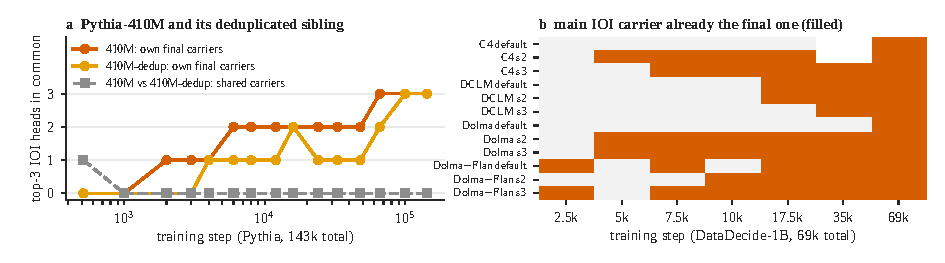
\includegraphics[width=\textwidth]{figures/fig2_lineage}
\caption{Carriers along pretraining.
(a) Number of each Pythia-410M model's final top-three IOI carriers already among its top three (solid), and number of top-three carriers shared by the two siblings (dashed).
(b) Twelve DataDecide-1B runs (four corpora $\times$ three initializations): filled where the current main IOI carrier is the run's final main carrier.}
\label{fig:lineage}
\end{figure*}

Before that, during pretraining, the carriers move (Figure~\ref{fig:lineage}).
In Pythia-410M, IOI appears at step 3000; head \head{11.4} becomes the strongest carrier at step 2000 and stays so, while the second and third places change among name movers until step 66k, after which the final top three are in place.
Its deduplicated sibling settles on a different main carrier, \head{12.12}, by step 6k and completes its final top three at step 100k.
From the moment carriers appear, the two siblings share none of their top three, while their attention roles start at a correspondence of 0.79 and diverge slowly to 0.47.
In DataDecide-1B, the head that carries IOI when the behaviour first appears is still the main carrier at the end of training in five of twelve runs; in the other seven, another member of the same class takes over later in pretraining.

Carrier assignment is thus an outcome of a run's own training.
Siblings begin from the same coordinate system, the members of each functional class compete for the task while the corpus is being learned, and the winner is kept once pretraining is over.
This explains the two halves of Figure~\ref{fig:carryover}: siblings have each been through their own competition, descendants inherit its result.

\section{Data interventions and the competition among candidates}
\label{sec:masking}

\begin{figure*}[t]
\centering
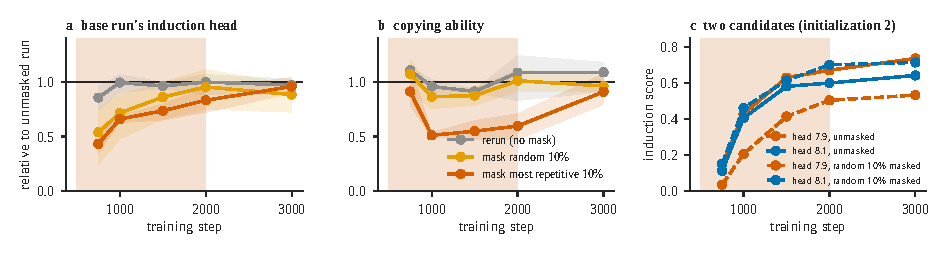
\includegraphics[width=\textwidth]{figures/fig3_masking}
\caption{Masking training data while induction heads emerge (shaded: steps 500--2000) in controlled 12-layer models from three initializations.
(a) Induction score of the unmasked run's strongest induction head, relative to the unmasked run (mean and range over initializations); (b) copying ability (loss reduction on the repeated half of random sequences), relative.
(c) Initialization 2 has two near-equal candidates; masking a random 10\% of sequences hands the role to the second one at emergence, and it keeps it.}
\label{fig:masking}
\end{figure*}

The competition among candidates also determines what a training-data intervention does to a single head.
Training-data attribution identifies the data that create a component by removing data, retraining, and reading out the same head \citep{chen2026mechanistic}.
We run such interventions with controlled pretraining, where the initialization and the data order are fixed and only the intervention differs (Figure~\ref{fig:masking}).
From three initializations we mask the loss of 10\% of the sequences during steps 500--2000, the window in which induction heads emerge: either the most repetitive sequences, the data that most accelerate induction heads \citep{chen2026mechanistic}, or a random 10\%.

When one head leads the role, the intervention delays that head.
Masking the most repetitive data lowers the strongest head's induction score to 36--55\% of the unmasked run at step 750 and copying ability to about half at step 1000; afterwards both recover, and at step 3000 the strongest induction head is the same head in all three initializations.
A rerun of the unmasked configuration reproduces the same head in all three.
Here a drop in the head's score is a delay of the mechanism, and a single-head readout measures exactly that.

When two heads compete, a small change in the data decides the winner.
In initialization 2, heads \head{7.9} and \head{8.1} rise together and \head{7.9} stays slightly ahead in the unmasked run and in its rerun.
Masking a random 10\% of the sequences lets \head{8.1} lead from the moment induction appears, and it keeps the role: at step 3000 the original head scores 72\% of the unmasked run while the strongest induction score (97\%) and copying ability (92\%) are intact.
A readout of \head{7.9} alone would report a weakened mechanism where the mechanism has moved.
Induction heads thus show, in miniature and under full control, the pattern of the IOI carriers: a role with one leading candidate stays on its head, and a role with several candidates goes to whichever candidate the run's data favour when the role is formed.

\section{Related Work}

\paragraph{Universality and stability of components.}
Circuits are consistent in their algorithm across training and scale while components change \citep{tigges2024llm}; attention heads are unstable across seeds, most in middle layers \citep{bali2026quantifying}; positional consistency across Pythia seeds is limited \citep{trott2025generalizability}; and representations of independently trained networks share structure up to rotation or permutation \citep{li2016convergent,kornblith2019similarity,ainsworth2023git}.
Seed variants such as PolyPythias \citep{vanderwal2025polypythias} and MultiBERTs \citep{sellam2022multiberts} change initialization and data order together.
We separate initialization from data, and separate attention roles from causal carriers, which explains why components agree among siblings in one sense and not in the other.

\paragraph{Mechanisms after further training.}
Fine-tuning reuses and enhances the circuits of the base model \citep{prakash2024finetuning}.
We show this for a full public lineage, through midtraining on new mixtures, SFT, DPO and instruction tuning, and contrast it with siblings trained separately.

\paragraph{Training data and components.}
Influence-based attribution traces heads to training samples and verifies the attribution by retraining \citep{chen2026mechanistic}; data properties such as burstiness shape when in-context learning emerges \citep{chan2022data}.
Our controlled masking shows when such interventions delay the same head and when they move the role to another candidate.

\paragraph{Reliability of circuit measurements.}
Circuit scores vary across inputs and methods \citep{meloux2026statistical}, and redundant heads repair ablations \citep{mcgrath2023hydra}.
Split-half reliability of every head map, and its correction of cross-model correspondence, make comparisons of causal maps between models interpretable.

\section{Discussion}
\label{sec:discussion}

\paragraph{When to carry a finding over.}
Our results give a rule for reusing head-level findings.
Along a training lineage, from a checkpoint to its continued pretraining, midtraining, SFT, DPO and instruction-tuned descendants, the named carriers can be reused directly.
Between siblings that share an initialization, attention-role labels can be reused directly, and the carriers of a task are localized again with a causal readout.
Between independently initialized models, the layer and the algorithm carry over.
For data interventions, a single-head readout tracks the mechanism when one candidate leads the role; reading out the strongest head of the role and the behaviour as well covers the case in which candidates compete.

\paragraph{What the coordinate system is.}
The initialization does not choose the carriers; it chooses where each role can live.
Every member of a functional class is a candidate for the task, and the run's own data decide which candidate wins.
This places the variation that \citet{tigges2024llm} and \citet{bali2026quantifying} observe across seeds at a definite point: in the competition among candidates during pretraining, not in the coordinates of the roles, which the initialization sets, and not in later training, which keeps the outcome.

\section*{Limitations}
We trace one task circuit, IOI, through causal carriers and nine roles through attention and weights; extending the carrier analysis to circuits for factual recall and in-context learning is the natural next step.
The public lineages we use reach 12B parameters in Pythia and 1B in OLMo~2, and the controlled interventions use 12-layer models, so the same measurements on larger lineages with released midtraining and post-training stages would extend the rule to current frontier pipelines.

\section*{Ethical Considerations}
This work analyses publicly released models and data. It reports lineage mismatches in public checkpoints so that users of these suites can compare the models they intend to compare.

\bibliography{refs}

\appendix

\section{Lineage of public checkpoints}
\label{app:audit}
Head layouts identify which checkpoints share an initialization, and we confirmed each case with the weights.
\begin{enumerate*}[label=(\roman*)]
\item In DataDecide-1B, six runs were trained from initializations other than the one their seed label names; they form three pairs that share an unregistered initialization (step-0 weight correlation 0.000 with the labelled seed; step-2500 weights correlate within each pair as strongly as true siblings). We exclude them from all sibling analyses.
\item The PolyPythias 160M \texttt{weight-seed} variants were trained from the standard initialization: their step-1 weights correlate 1.0 with the standard step 0, although their released step-0 files differ.
\item The released final checkpoint of Pythia-2.8B-deduped is nearly identical to Pythia-2.8B (weight correlation 0.99), so this pair cannot serve as a same-initialization, different-data pair.
\item The \texttt{main} revision of OLMo-2-0425-1B comes from a different training run than its released stage-1 and stage-2 checkpoints and its SFT, DPO and Instruct models: a layer-5 query matrix correlates 0.000 with every stage checkpoint and with the Instruct model, while the Instruct model correlates 0.976 with the end of midtraining, and the head layouts agree accordingly. Lineage analyses should start from the stage-2 checkpoints.
\end{enumerate*}

\section{Role definitions}
\label{app:roles}
Induction: attention from the second copy of a repeated random block to the token after the earlier occurrence.
Previous token, current token, two tokens back: attention to positions $t-1$, $t$, $t-2$ on natural text.
Attention sink: attention to position 0.
Knowledge retrieval: attention from the final prompt token to the answer entity in knowledge-conflict prompts.
Duplicate token: attention from the second copy of a random block to the same token's first occurrence.
Delimiter: attention mass on punctuation and newline tokens.
OV copying: $\sum \mathrm{Re}\,\lambda / \sum |\lambda|$ over the eigenvalues of the full OV circuit.
All attention roles are averaged over two halves of their inputs; split-half reliabilities are 0.98 or higher.

\section{Controlled pretraining}
\label{app:controlled}
The models have 12 layers, 12 heads, width 768 and a 50k vocabulary, and are trained on C4 with sequences of 512 tokens, batches of 64 sequences, AdamW (learning rate $10^{-3}$, 300 warm-up steps, cosine decay over 10k steps), for the first 3000 steps from three initializations with one data order.
Masking sets the loss weight of the selected sequences to zero for steps 500--2000 and leaves the data order unchanged.
A sequence's repetition score is the share of tokens whose preceding bigram occurred earlier in the sequence followed by the same token; the masking threshold is the 90th percentile on C4 (0.08).
Random masking selects 10\% of sequences with a separate random generator.

\end{document}
